%\documentclass{article}
%\documentclass[aip,jcp,amsmath,amssymb,reprint]{revtex4-1}

\documentclass[conference]{IEEEtran}
\IEEEoverridecommandlockouts
% The preceding line is only needed to identify funding in the first footnote. If that is unneeded, please comment it out.
\usepackage{cite}
\usepackage{amsmath,amssymb,amsfonts}
%\usepackage{algorithmic}
\usepackage{graphicx}
\usepackage{textcomp}
\usepackage{xcolor}
\def\BibTeX{{\rm B\kern-.05em{\sc i\kern-.025em b}\kern-.08em
		T\kern-.1667em\lower.7ex\hbox{E}\kern-.125emX}}


\usepackage[utf8]{inputenc}
%\usepackage[ruled,vlined]{algorithm2e}
\usepackage{algpseudocode}
\usepackage{algorithm}
\usepackage{amsmath}
\usepackage{amssymb}

\newcommand{\pluseq}{\mathrel{+}=}
\newcommand{\minuseq}{\mathrel{-}=}
\newcommand{\asteq}{\mathrel{*}=}
\renewcommand{\algorithmiccomment}[1]{\hfill$\triangleright$\textit{#1}}

\title{CS7642 Project 2 -- Solving LunarLander problem with Double Deep Q-Learning}
\author{Qinghui Ge}
\date{January 2020}

\begin{document}
	
	\maketitle
	
\begin{abstract}
	In this report, I will demonstrate using Double Deep Q-Learning (DDQL) to solve a model reinforcement learning problem -- LunarLander. 
\end{abstract}
	
\section{introduction to LunarLander}
In the LunarLander problem, the goal is to control a lander to land between two flags without crash. The state of the lander is specified by 8 numbers: ($x$, $y$, $v_x$, $v_y$, $\theta$, $v_\theta$, $leg_L$, $leg_R$).
$x$ and $y$ are coordinate of the lander position. $v_x$ and $v_y$ are velocity components on the x and y axes. $\theta$ and $v_\theta$ are the angle and angular velocity. $leg_L$ and $leg_R$ are binary values indicating whether the left or right leg of the lander is touching the ground. There are four possible actions: do nothing, fire left orientation engine, fire main engine, fire right orientation engine.

In opengym's implementation of LunarLander environment, moving the lander from top of the screen to landing pad receives 100-140 points; the same amount would be penalized if lander landed outside the designed area; crash or successful landing get -100 and +100 points, respectively; each leg ground contact is worth +10 points; firing the main engine incurs a -0.3 point penalty for each occurrence. A decent landing policy should receive +200 points on average. Designing a reward function like above is a useful technique called reward shaping in reinforcement learning, which is supposed to give more frequent feedback to the learner and make the learning process easier. 

\section{Deep Q-Learning}
In basis Q-Learning, the value of each state-action pair (expected reward if an agent is in state s and performs action a, and then continues playing until the end of the episode following some policy $\pi$) is stored in a matrix Q(s,a) -- the Q-table. The Q-Learning procedure keeps updating the Q-table using the experiences so that the Q-values converge to it's optimal value. 

Keep a record of the entire Q-table can be impractical if the number of state and actions are large, or if the state or action is continuous, as in the case of LunarLander. In case of continuous state and discrete action space, Deep Q-Learning (DQL) uses a neural network to generate approximate Q-values for any state on the fly (see Fig. for a comparison between Q-Learning and Deep Q-Learning). Instead of updating the Q-table, the learning process updates the neural network that predict Q values.

At time step $t$, the action $a_t$ can be selected from $\epsilon$-greedy algorithm using the prediction of neural network $Q$ of state $s_t$:

\begin{algorithm}[h!]
	\caption{$\epsilon$-greedy}
	\begin{algorithmic}
		\Function{$\epsilon$-greedy}{s, Q, $\epsilon$}
		\If {random\_number()  $<\epsilon$}
		\State return random action
		\Else
		\State return $argmax_a Q(s, a)$
		\EndIf
		\EndFunction
	\end{algorithmic}
	\label{algo:seq}
\end{algorithm}

If we know the ground truth $Q_{true}$, we can simply update the neural network parameter $\omega$ by minimize some Loss function such as L2 loss/MSE:
\begin{equation}
Loss = \frac{1}{N_sN_a}\sum_{s,a}(Q_{true}(s, a) - Q_\omega(s_t, a_t))^2
\end{equation}
However, unlike supervised learning, we do not know the ground truth $Q_{true}$, instead we use Bellman equation to estimate $Q_{true}$, or the TD-target. The TD-error of neural network with parameter $Q_w$ is estimated by:
\begin{align}
Error &= Q_{target} - Q_\omega(s_t, a_t)  \\
&= R(s_t, a_t) + \gamma * max_a Q_{\omega}(s_{t+1}, a) - Q_\omega(s_t, a_t)
\end{align}
The estimation of $Q_{target}$ would in turn depends on $Q_\omega$, which makes the training unstable. To combat this problem, Deep Q-Learning method introduces another target network $Q^t$. $Q^t$ is used to compute the TD-target, while $Q$ is used to determine the 
$\epsilon$-greedy action $a_t$:
\begin{equation}
Q_{target} = R(s_t, a_t) + \gamma max_a Q^t_{\omega'}(s_{t+1}, a)
\label{eq:tdtarget}
\end{equation}
Note 

The target network $Q^t$ has the same architecture as the prediction network $Q$, but its parameter $\omega'$ is updated in a slower fashion than $Q$. For example, update $Q^t$ for every K times after $Q$ is updated, or soft-update $Q^t$ with some parameter $\tau<1$:
$Q^t \leftarrow \tau Q + (1-\tau) Q^t$. This way, the target is kept frozen for some period and the training is more stable.

Another technique used in Deep Q-Learning is the replay buffer. In basic Q-Learning, Q values are updated for every observed state-action pair. This would be inefficient if we want to apply stochastic gradient decent (SGD) to update the weights of network $Q$. Further, SGD works best when the samples in each batch is independent, which is unlikely for state-action pairs coming from a same episode. Thus DQL use a replay buffer to store accumulated experiences in memory. Then for each time step, a a batch of samples can be randomly draw from the buffer to feed into SGD. Each experience contains the following information: [state ($s_t$), action ($a_t$), reward ($R_t$), next\_state ($s_{t+1}$), done(end of episode)].

\section{Double Q-Learning}
In basic Q-Learning and Deep Q-Learning, the max operator in computing TD-target(Eq.\ref{eq:tdtarget})  uses same value for evaluating and selecting an action. This causes a bias that the actions whose Q-values are overestimated are more likely to be selected. For basic Q-Learning, van Hasselt et.al proposed using two independent Q-tables to decouple evaluation and selection. In each iteration, one Q-table is used to select the action, another is used to evaluate the Q-value, and the choice is made by random 50\%-50\% chance. This is the original Double Q-Learning algorithm.

\section{Double Deep Q-Learning}
For Deep Q-Learning, van Hasselt et.al suggest using the target network to partially decouple evaluation and selection. This introduce a minimal change on top of the existing Deep Q-Learning algorithm without introducing another network. In this Double Deep Q-Learning algorithm, instead of taking $max$ of target network $Q^t$, we first determine the greedy action with $Q$, then evaluate $Q^t$ at the greedy action:
\begin{align}
& Q_{target} = R(s_t, a_t) + \gamma Q^t_{\omega'}(s_{t+1}, a^*) \\
& a^* = argmax_a Q_\omega(s_{t+1}, a)
\end{align}

Summarizing the above, we follow Algorithm \ref{algo:ddql} to implement Double Deep-Q Learning in this work. Note in actual implementation, the for loop in each batch is vectorized to improve computational efficiency.

\begin{algorithm}[h!]
	\caption{Double Deep-Q Learning}
	\begin{algorithmic}
		\Function{update}{$Q$, $Q^t$, buffer}
		\State batch = random\_choice(buffer, batch\_size)
		\For {each sample=[$s_t$, $a_t$, $R_t$, $s_{t+1}$, done] in batch}
			\If {done}
				\State $Q_{target}(s_t, a_t) = R_t$
			\Else
				\State $a^* = argmax_a Q_(s_{t+1}, a)$
				\State $Q_{target}(s_t, a_t) = R_t + \gamma * Q^t_a(s_{t+1}, a^*)$
			\EndIf
			\State for other $a\neq a_t$: $Q_{target}(s_t, a) = Q(s_t, a)$
		\EndFor
		\State update $Q$: one step of gradient decent using $x=s_t(batch)$, $y=Q_{target}(batch)$.
		\State update $Q^t$: $Q^t \leftarrow \tau Q + (1-\tau) Q^t$
		\EndFunction
		\\
		\Function{Double Deep-Q Learning}{ }
		\State initialize $Q$, $Q^t$ to have the same random weights.
		\State initialize replay buffer with max\_size
		
		\For {each episode}
			\State reset environment
			\For {step t in episode}
				\State $a_t = \epsilon$-greedy(s, Q, $\epsilon$)
				\State take action $a_t$, observe $s_{t+1}, R_{t}$, done
				\State add [$s_t$, $a_t$, $R_t$, $s_{t+1}$, done] to replay buffer
				\State update($Q$, $Q^t$, buffer)
			\EndFor			
			\State $\epsilon \asteq decay$
		\EndFor
		\EndFunction
	\end{algorithmic}
	\label{algo:ddql}
\end{algorithm}


There are a number of hyperparameters involved in DDQL:
\begin{enumerate}
\item $\epsilon$ / $decay$. In $\epsilon$-decay algorithm, $\epsilon$ controls explore rate. With larger $\epsilon$, random action is choose more frequently and thus more exploration, while small $\epsilon$ leads to greedy action. $\epsilon$ can be annealled with a decay factor, such that exploration is favored in earlier episodes, as training goes on, the algorithm shift towards more exploitation.
\item max\_size of replay buffer. The replay buffer is set to have a max\_size. When max\_size is reached, most recent experience will overwrite oldest experience. The size should be neither too small nor too large. A small buffer will have a lot of correlated samples and the training will be unstable; large buffer may contain out-dated sample computed from less optimized $Q$ that leads to slow convergence.
\item $\tau$. The parameter controls soft-update. For larger $\tau$, the target network $Q^t$ is more update-to-date with $Q$, so the training may become unstable. For small $\tau$, updates of $Q^t$ is lagged behind $Q$, this could make training stable but converge slower.
\item $\gamma$ the discount factor as in regular Q-learning.
\item Neural-net related hyperparamters, such as network structure, loss function, optimizer, learning rate $lr$, batch-size, etc.
\end{enumerate}
	
\section{Experiment  Results}
\subsection{Training Agent}
Using the following setting, we obtain a trained agent that is able to achieve +200 reward for an average of 100 episodes:
\begin{enumerate}
\item inital $\epsilon$=1, $decay$=0.995
\item max\_buffer\_size = 9600
\item $\tau$ = 0.001
\item $\gamma$ = 0.99
\item Neural Network with two hidden layers of 64 and 32 units, both using LeakyRelu activation. Output layer has $N_A$ (4 in the case of LunarLander) output numbers, using Linear activation. Adam optimizer with learning rate $lr=0.0005$ is used to minimize MSE loss. Batch\_size = 32 for sampling replay buffer.
\end{enumerate}
We train the agent for 1000 episodes, Fig. X shows the reward of each episode during training process. The moving average reward of 100 episodes reaches +200 at around 500 episodes. Afterwards the rewards can still be negative for certain episodes, although the moving average remains above +200 until the end. Using the weights obtained at the end of 1000 episodes, we can evaluate total reward of 100 independent episodes. The distribution of 100 rewards in show in Fig. X. We are able to achieve average total reward of 227, with standard deviation = 55.

\subsection{Effect of Hyperparameters}
Next we will study the effect of a few hyperparameters: learning rate $lr$, decay factor, $gamma$, and soft-update parameter $\tau$. Other parameters are kept the same though all experiments: initial $\epsilon=1$, batch\_size = 32 , max\_buffer\_size = 9600.

First, we retrain the agent at different learning rate: $lr = 0.005, 0.001, 0.0005, 0.0001$, with other parameters fixed. The learning curves of different learning rate are shown in Fig. \ref{fig:lr}. $lr = 0.001$ and $0.0005$ is able to achieve moving average reward $>200$ during training. For larger learning rate $0.005$, although it performs similarly at the beginning, the rewards does not improve to +200 later on. Small learning rate $0.0001$ learns slowly at the beginning, rewards decrease again towards negative in later episodes, as if the agent ``forget" what is has learned. 

	\begin{figure}
		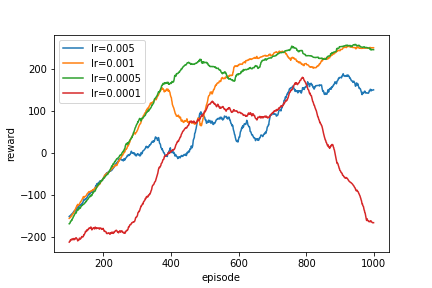
\includegraphics[height=2.5in]{figures/lr.png} 
		\caption{Effect of learning rate. Moving average reward of 1000 episodes for different $decay$ values during training process. $decay=0.995$, $\tau=0.001$, $\gamma=0.99$ for all runs. The moving average is evaluated with a window of 100 episodes.}
		\label{fig:lr}
	\end{figure}

We then turn to the decay rate for $\epsilon$-greedy algorithm. We experimented with $decay = 0.999, 0.995, 0.99, 0.95$. Smaller decay would make the training enter exploitation phase earlier, and the rewards can increase faster in the beginning. As show in Fig. \ref{fig:epsilon_decay}, in the first 100 episodes, the reward increase quickest for $decay = 0.95$, and slowest for $decay = 0.999$. However, without enough explore, the agent do not perform great in the long run: $\epsilon = 0.995/0.99$ out-performs $decay = 0.95$ in the end. Too large $decay$ is not idea either, for $decay = 0.999$, the learning becomes very slow, because the agent is unable to exploit the learned greedy actions.

	\begin{figure}
		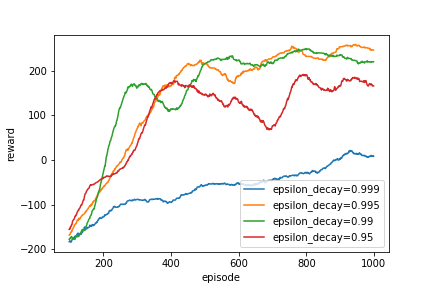
\includegraphics[height=2.5in]{figures/epsilon_decay.png} 
		\caption{Effect of epsilon\_decay. Moving average reward of 1000 episodes for different $decay$ values during training process. $\tau=0.001$, $lr=0.0005$, $\gamma=0.99$ for all runs. The moving average is evaluated with a window of 100 episodes.}
		\label{fig:epsilon_decay}
	\end{figure}
	
The soft-update parameter $\tau$ acts as a learning rate for the target network. In Fig. \ref{fig:tau}, we can see larger $\tau$ values like $\tau=0.005$ leads to more instability during the training process, as the target network is updated more aggressively. On the other hand small $\tau$ values like $\tau=0.0002$ and $\tau=0.0001$ will slow down the learning. $\tau=0.0005$ or $0.001$ achieves best performance by balancing the stability and learning efficiency, and are able to achieve moving average reward $> 200$ without too much fluctuation.

\begin{figure}
	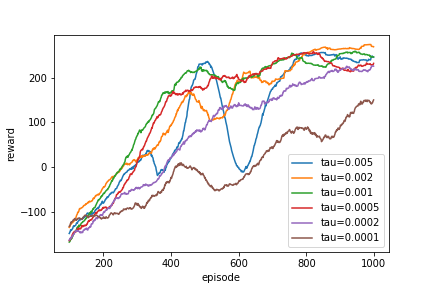
\includegraphics[height=2.5in]{figures/tau.png} 
	\caption{Effect of $\tau$. moving average reward of 1000 episodes for different $\tau$ values during training process. $decay=0.995$, $lr=0.0005$, $\gamma=0.99$ for all runs. The moving average is evaluated with a window of 100 episodes.}
	\label{fig:tau}
\end{figure}
	
Finally, we take a brief look at the discount factor $\gamma$. As the goal is to optimize the undiscounted reward during the entire episode, our intuition is $\gamma=1$ may yield the best results. However, interestingly the training seems to be less stable with $\gamma=1$. In Fig. \ref{fig:gamma}, we compare the four independent runs of $\gamma=1$ and $\gamma=0.99$. The learning curve for $\gamma=1$ has larger fluctuation, and the rewards can drop quickly to negative even though the initial training seems to be on the right track. Choosing $\gamma$ to be smaller than 1 partly alleviate the problem, as shown in the 4 runs of $\gamma=0.99$.

\begin{figure}
	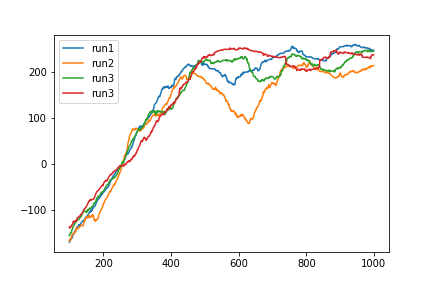
\includegraphics[height=2.5in]{figures/gamma099.png}  \\ 
	\centering (a) $\gamma=0.99$\\
	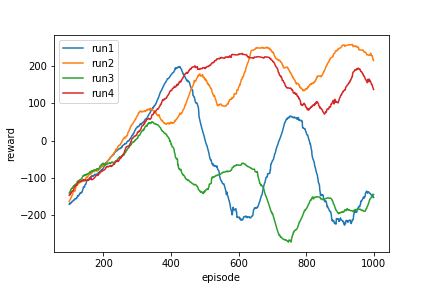
\includegraphics[height=2.5in]{figures/gamma1.png}  \\ 
	\centering (b)  $\gamma=1$
	\caption{Comparison between $\gamma=0.99$ (a) and $\gamma=1$ (b). Each graph shows the moving average reward of four independent runs of given $\gamma$ value, with $decay=0.995$, $lr=0.0005$, $\tau=0.001$. The difference between 4 runs of same $\gamma$ value comes from random seed settings. It is shown that $\gamma=0.99$ gives more stable learning curves.}
	\label{fig:gamma}
\end{figure}
	
\section{Discussion}
Training the agent with Double Deep Q-Learning is challenge in a few ways. The hyperparameters have to be carefully tuned to balance exploration and exploitation, stability and efficiency. With current hyperparameters set, I still experience in stability frequently, the training reward sometimes decrease a lot after reaching +200. We may consider stop the training once the reward reaches +200, or save the model weights though the way and pick the best weights afterwards. It is worth-noting the reward observed in the training curve is not exactly the test reward, because the training reward is computed with different networks in each episode, although they may be roughly correlated with each other. Ideally, we can obtain test-reward during the training process. However, this could be expensive because test-reward is evaluated by averaging 100 independent runs in order to get some statistical significance.

Currently we are keeping other parameters fixed while studying the effect of a given hyperparameter, it also would be interesting to explore the correlations between parameters. For example, the smallest learning rate $lr=0.0001$ performs poorly with $decay=0.995$, it is possible that we may want to increase the $decay$ value (slower decay, more exploration) to adapt to the slower learning rate.

Each training currently takes about 30 minutes on CPU for 1000 episodes, this makes massive hyperparameter searching difficult. Surprisingly the bottleneck is not updating the network weights, but using the network to predict next action, which is a step hard to be parallelized.

We also note that when using the opengym implementation of the environment, unless using the ``unwrapped" setting, the episode is going to be terminated at some max time step (1000 for LunarLander). In those unnatural termination, the Bellman equation for TD-Target should include the value of next state, rather than just reward. The results above were obtained without the tweak. Some initial trials with the modification did not give significant performance change. However, due to the randomness in the algorithm, we need more experiment (like the multiple runs for studying the effect of $\gamma$) to reach a solid conclusion. And we could monitor the frequency of reaching max time step to access the potential impact for this problem.

	
\bibliographystyle{IEEEtran}
\bibliography{reference}

\end{document}
